\documentclass[12pt,fleqn]{article}
\usepackage{xiiiemc}
\usepackage{natbib}
\usepackage{fancyhdr}
\usepackage{color}
\usepackage{wallpaper} 
\usepackage{titlesec}   %% Define space between paragraph e section
\usepackage{float} 	%% Use to fix Figure or Table: ex: \begin{table}[H]
%%%%Don't edit this block. It reduces the spacing between the lines of the references
\let\OLDthebibliography\thebibliography
\renewcommand\thebibliography[1]{\OLDthebibliography{#1} \setlength{\parskip}{0pt}\setlength{\itemsep}{0pt plus 0.3ex}}

%%-----------------------------------------------EDIT-----------------------------------------------
\title{INSTRUCTIONS FOR PREPARATION AND SUBMISSION OF PAPERS FOR PUBLICATION IN THE PROCEEDINGS OF XXI ENMC / IX ECTM}

%%-----------------------------------------------EDIT----------------------------------------------
\author
    {\rm \begin{tabular}{l} 
    \textbf{First Author}$^{1}$ - {\textnormal e-mail}\\%
    \textbf{Second Author}$^{2}$ - {\textnormal e-mail}\\
    \textbf{Third Author}$^{3}$ - {\textnormal e-mail}\\
    {\fontsize{11}{0}\selectfont $^{1}$Universidade do Estado do Rio de Janeiro, Instituto Politécnico - Nova Friburgo, RJ, Brazil}\vspace*{-0.05cm} \\
    {\fontsize{11}{0}\selectfont $^{2}$Institut Polytechnique de Grenoble - Grenoble, France}\vspace*{-0.05cm}\\
    {\fontsize{11}{0}\selectfont $^{3}$Universidade Estadual de Santa Cruz, Campus Soane Nazaré de Andrade - Ilhéus, BA, Brazil}
  \end{tabular}}
%%----------------------------------------------------------------------------------------------

\fancypagestyle{firspagetstyle}
{
	\lhead{}
	\fancyhead[C]{%
		
\includegraphics[width=0.75\linewidth]{logo}\\%
		{\scriptsize \fontfamily{phv}\fontseries{b}\selectfont \color[rgb]{0.45,0.45,0.45}
		08 a 11 de Outubro de 2018\\
		Instituto Federal Fluminense\\
		Búzios - RJ\\
	    }
	}
	\renewcommand{\headrulewidth}{0.0pt}
	\fancyfoot[C]{\footnotesize \parbox{15cm} {\centering  \fontsize{7.5}{0}\selectfont \it Anais do XXI ENMC – Encontro Nacional de Modelagem Computacional e IX ECTM – Encontro de Ciências e Tecnologia de Materiais,  Búzios, RJ – 08 a 11 Outubro 2018}} % \ttfamil
	\rhead{}
}


\begin{document}
\maketitle

\thispagestyle{firspagetstyle}

\fancyhead[L]{\footnotesize{\fontsize{7.5}{0}\selectfont \it XXI ENMC e IX ECTM\\
	08 a 11 de Outubro de 2018\\
	Instituto Federal Fluminense – Búzios - RJ\\}}
\renewcommand{\headrulewidth}{0.0pt}
\fancyfoot[C]{\footnotesize \parbox{15cm} {\centering  \fontsize{7.5}{0}\selectfont \it Anais do XX ENMC – Encontro Nacional de Modelagem Computacional e VIII ECTM – Encontro de Ciências e Tecnologia de Materiais,  Nova Friburgo, RJ – 16 a 19 Outubro 2017}} % \ttfamil
\rhead{}

\begin{abstract}
This document-template provides detailed instructions for preparing and submitting a paper to XXI ENMC - National Meeting on Computational Modeling and IX ECTM -Meeting on Materials Science and Technology. Please follow these instructions: a) type the body of the paper in a single column; b) use 5 to 10 A4-size pages (21cm $\times$ 29.7cm), each formatted with 2.5cm margins on all sides except at the top of the page (do not print any border around the text and do not insert page numbers); c) use 12 pt Times New Roman throughout, except on affiliation identification; d) type up to 200 words in the abstract, in italics; e) always use single-spaced lines, justified alignment; f) cite references by name (year) and list in alphabetical order by author last name at the end; g) supply good quality figures/photographs (black and white only); h) define all symbols as they appear in the text; i) use only SI units. The paper may be written in English, Portuguese or Spanish.
\end{abstract}

\keywords{\em{First keyword, Second keyword, Third keyword (up to 5 keywords) }}

\pagestyle{fancy}

\section{INTRODUCTION [Times New Roman 12pt, all capital letters, bold]}
The Proceedings of XXI ENMC/IX ECTM, including the full versions of all papers to be presented at the meeting, will be published in digital media. Therefore, it is extremely important that you prepare the PDF digital version of your contribution in accordance with the present instructions. The file size must be less than 4 MB.

The Editorial Committee will evaluate all submitted papers.

\section{TYPING INSTRUCTIONS}
The paper must be written in English, Portuguese or Spanish. {\it If written in Portuguese or Spanish, a translation of title, abstract and keywords into English must be provided at the end of the paper (after the reference list)}.

% \ \ \ \
\newpage %
\subsection{Paper length}
The full paper including figures and tables must have at least 5 pages, but is limited to 10 A4-size pages (21 cm x 29.7 cm). Please limit your paper by writing concisely, rather than by reducing figures or tables to a size at which symbols/labels become difficult to read.

\subsection{Page format}
Each A4-size page should be formatted with 2.5 cm margins on all sides, except at the top. This defines the printable area. Inside this area, the text must be arranged in a single column. Please do not print any border around the text and do not insert page numbers.

The final paper should look like this document.

\subsection{General text specifications}

The paper must be typed using 12 pt Times New Roman throughout the text, as in the present document. This includes title, headings, and figure and table captions.

\vspace{0.5cm} % Example spaces

\textbf{\textit{Paper title.}} The title should be in boldface type, all capital letters and centered on the page and must not exceed three lines. It should be single spaced if longer than one line. Skip one line (12 pt) between the title and the first author.

\vspace{0.5cm} % Example spaces

\textbf{\textit{Author(s) and affiliation.}} Type authors names in boldface type, flush left, one per line, including first name, middle and last name, followed by the e-mail address (not boldfaced). After the name put in superscript the number, related to the affiliation. The authors names should be followed by the corresponding affiliation, which should be in regular type (neither boldfaced nor italicized). After presenting affiliations should skip two lines (24 pt) between the last affiliation and the abstract.

\vspace{0.5cm} % Example spaces

\textbf{\textit{Abstract and keywords.}} Type the heading \textbf{\textit{Abstract.}} in boldface italics, flush left, followed by a period. On the same line, type the abstract in italics, justified alignment. The abstract should be no longer than 200 words. Skip one line, then type the heading \textbf{\textit{Keywords:}} (don't forget the colon) in boldface italics, flush left and type 3 to 5 keywords, separated by commas, with only the first letter of each keyword capitalized. Skip two lines (24 pt) between the keywords and the body of text.

\vspace{0.5cm} % Example spaces

\textbf{\textit{Headings.}} Type a first-level head (section) in all capital letters, boldface type, flush left. Begin by typing the Arabic number followed by a period, then type the head title 0.75 cm (or 7 blank spaces) from the left margin. Leave one blank line above and one below this head. 

For a second-level head (subsection), capitalize only the first letter, using boldface type, flush left. Begin by typing the double number, then type the sub-head title 0.75 cm from the left margin. Leave one blank line above and one below this head. 

Do not number third-level heads (sub-subsection). Use boldface italics, capitalizing only the first letter and indenting 0.75 cm from the left margin. Follow it by a period and start the text immediately. Leave one blank line above this head.

\vspace{0.5cm} % Example spaces
% 
\textbf{\textit{Body of text.}} The text should be typed using single-spaced lines and justified alignment. Start each paragraph 0.75 cm from the left margin and allow no space between paragraphs.

\subsection{Equations, symbols and units}
Indent an equation 1 cm (or 10 spaces) from the left margin. Number it with an Arabic number enclosed in parentheses, placed flush right. Allow one blank line above and one below each equation. For example:
\begin{equation}
\vec{q}_{r}=-4\pi r^{2}k\frac{dT}{dr}
\label{eq1}
\end{equation}
%%%here space

When referring to an equation in the text write Eq. (1), except at the beginning of a sentence, where Equation (1) should be used. 

Symbols should be italicized throughout the text. Define all symbols as they appear in the text. A nomenclature section is not necessary.

All data, including those shown in tables and figures, must be reported in SI units. 

\subsection{Figures and tables}
Figures and tables should be inserted as close as possible to their mention in the text. Enclosed text and symbols must be clearly readable; avoid small symbols. Supply good quality pictures and illustrations.

Figures and tables and their captions should be centered in the text. Place figure caption below the figure, leaving one blank line between them. Place table title above the table, also leaving one blank line between them. Leave one blank line between the table or figure and the adjacent text. Color figures can be used.

Number figures and tables consecutively using Arabic numerals (e.g., Figure 1, Figure 2, Table 1, Table 2). Refer to them in the text as Table 1 and Fig. 1 (except at the beginning of a sentence, where Figure 1 should be used).
% TABLE EXAMPLE
\begin{table}[H] % !htbp 
\caption{Input parameters}
\vspace{12pt}
\centering{}
\begin{tabular*}{\textwidth}{@{\extracolsep{\fill}}ccc|cc}        % {0.8\textwidth}
\hline 
Method LJ & Configuration && Method R2W & Configuration\tabularnewline
\hline 
$k_1$ (W/mK)  & $[0,0; 0,1]$ && $k_1$ (W/mK) & $[0, 0; 0,1]$\tabularnewline
\hline 
$k_2$ (W/mK) & $[0,0; 0,1]$ && $k_2$ (W/mK) & $[0, 0; 0,1]$\tabularnewline
\hline 
$n$ & $1,0$ && $n$ & $1,0$\tabularnewline
\hline 
\end{tabular*}
\end{table}

\begin{figure}[!htbp] %h or !htbp
\vspace{-2pt}
\begin{center}
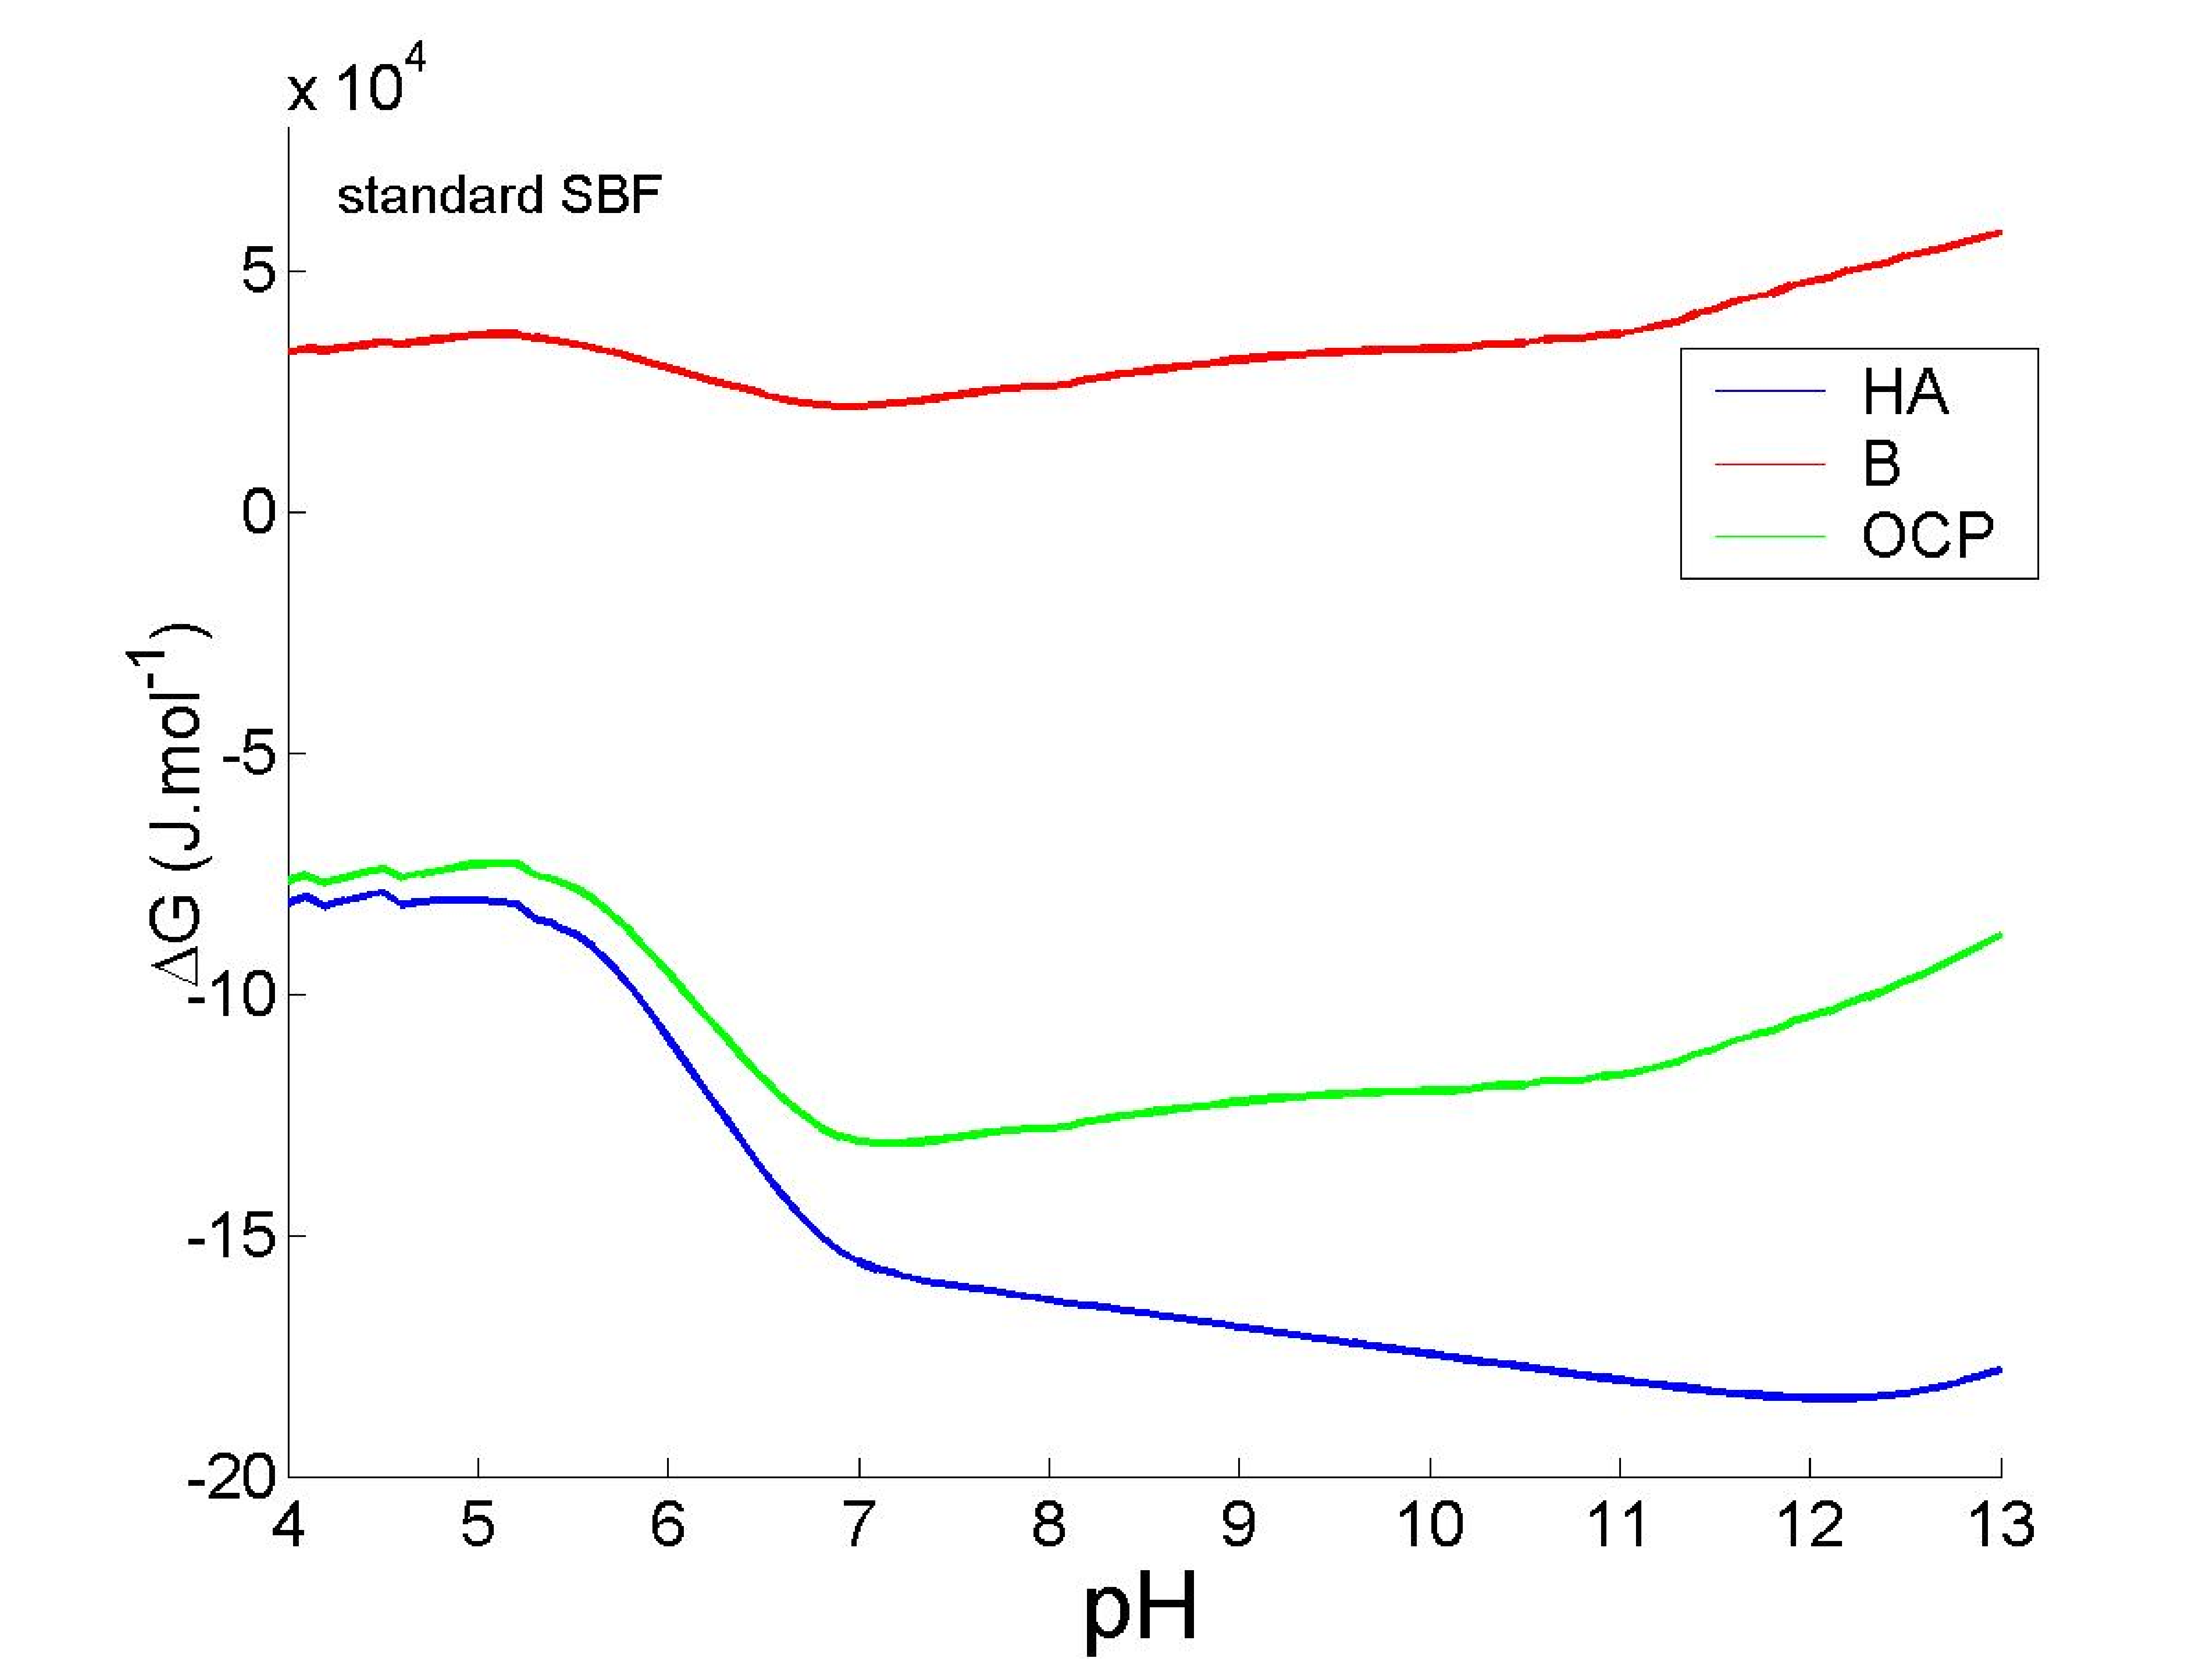
\includegraphics[height=6.7cm,width=9cm]{figura_1}%
\caption{Gibbs free energy variations: simulated results.}
\label{fig1}%
\end{center}
\end{figure}

Label coordinates in plots and add the corresponding units. Similarly, label columns/rows in tables and add the units.

\subsection{Permission}
You are responsible for making sure that you have the right to publish everything in your paper. If you use material from a copyrighted source, you may need to obtain permission from the copyright holder.

\section{CALL TO REFERENCES IN THE BODY OF TEXT}
References should be cited in the text by name last (year) or (last name, year). For example: ``In a recent work, Jones et al. (2005) proposed ...,'' or ``In a recent work (Devlou \& Zaparolli, 2013), it is suggested ... .''

References must be listed in alphabetical order at the end of the paper. Type the word \textbf{REFERENCES} in all capitals, boldface type from the left margin, skip one line and type the reference list. In each reference, indent all lines 0.75 cm except the first line, which starts directly at the left margin. Each reference must be cited in the text. In the section REFERENCES is presented an example of a reference list including a journal article, a report, an edited book, proceedings, a dissertation and a book.

\section{CONCLUSIONS}
This section should be included and need to show the main contributions of the paper in a briefly form.

\subsection*{\textit{Acknowledgements}}
This section should be positioned between the end of the text and the reference list. Type \textbf{\textit{Acknowledgements}} in boldface italics, skip one line of space and type the text in regular type.


% ------------------------------------------------------------------------
\begin{thebibliography}{99}
\fontsize{11}{0}\selectfont
\bibitem[Aznar \& Pessoa, 1994]{Aznar94}
Aznar, M., Pessoa, F.L.P. and Silva Telles, A. (1994), ``Vapor-Liquid Equilibria of Mixed Solvent-Salt Systems using a MHV2 Model with the Wilson Equation'', {\em X Congresso Brasileiro de Engenharia Química}, São Paulo, vol 1, 38-43.

\bibitem[Freitas et~al., 2008]{Freitas08}
de Freitas, G.C.S.; Peixoto, F.C.; Vianna Jr, A.S. (2008), Simulation of a thermal battery using Phoenics. Journal of Power Sources, 179, 424-429. 

\bibitem[Duarte, 1999]{Duarte99}
Duarte, C.S.A. (1999), {\em Equilíbrio Líquido-Líquido em Sistemas contendo Polímero e Eletrólito: Água/ Polietileno-glicol/Fosfato}, Laboratório de Equilíbrio de Fases, FEQ/UNICAMP, Campinas.

\bibitem[Fredenslund, 1993]{Fredenslund93}
Fredenslund A. e Sorensen, J.M. (1993), ``Group Contribution Estimation Methods'', in {\em  Models for Thermodynamic and Phase Equilibria Calculations}, S.I. Sandler (ed.), Marcel Dekker, Inc., New York.

\bibitem[Silva, 2005]{Silva2005}
Silva, L.F. (2005), ``{\em Predição de Pontos Críticos de Misturas Termodinâmicas}'', Tese de Doutorado, IPRJ/UERJ, Nova Friburgo.

\bibitem[Krevelenm, 1990]{Krevelen90}
Van Krevelen, D.W. (1990),{\em ``Properties of Polymers. Their Correlation with Chemical Structure, Their Numerical Estimation and Prediction from Additive Group Contribuition}'', 3º ed., Elsevier, Amsterdam.
\end{thebibliography}
\vspace*{-0.1cm}
\section*{APPENDIX A}
This section, if necessary, must be included here.

\vspace{0.5cm} % Example spaces

For Papers written in Portuguese or Spanish a translation of title, abstract and keywords into English must be provided after the Appendix using the same format for title, abstract and keywords presented in the first page of the template.
% ------------------------------------------------------------------------

%For papers written in Portuguese or Spanish.

%\begin{center}
%  TITLE IN ENGLISH
%\end{center}

%\def\abstractname{Abstract}%

%\begin{abstract}
%   Abstract in english
%\end{abstract}

%\keywords{\em{Keywords in english}}

\end{document}
